\section{Writing}

\lettrine{C}{lear} and concise writing is critical in science to convey research, making it a paramount skill to exercise. 
This section outlines advice, tips, and suggestions to consider when writing. 
The writing instruction provided is in no way conclusive, however, it is the author's hope that this document will be developed through time to ease students into the expectations of academic writing. 
Sources that go more in-depth on writing instruction include work by \citeauthor{natureWritingTips} \cite{natureWritingTips}, \citeauthor{writingSpringer} \cite{writingSpringer}, and \citeauthor{writingAIAA} \cite{writingAIAA}.

\subsection{Document Setup}

The most important thing to consider before even beginning to write is \textit{what are the expectations}. 
Every technical writing conference/journal/thesis will have a set of formatting requirements \cite{writingAIAA,writingThesisUofC}. 
Review these requirements \textbf{before} writing to save time re-formatting everything later. 
These organizational formatting requirements are the be-all-end-all to discussions about formatting, the document must align with the requirements. 

\subsubsection{Tense}

Tense is a common simple mistake that is easily correctable by considering the intent of the information. Tense is determined by what the sentence is describing \cite{natureWritingTips}, common sentence types and their associated tense are presented in \Cref{tab:tenseBasedOnSentence}. 

\begin{table}[hbt!]
	\centering
	\begin{threeparttable}[b]
		\caption{How tense changes based on the intent of the sentence \cite{natureWritingTips}. \label{tab:tenseBasedOnSentence}}
		\begin{tabular}{cc}
			\toprule
			\textbf{Sentence Describes} & \textbf{Tense} \\ \midrule
			Work done & \multirow{3}{*}{Past} \\
			Work reported &  \\
			Observations &  \\ \midrule
			General truths & \multirow{2}{*}{Present} \\
			Atemporal facts &  \\ \midrule
			Perspectives & Future \\ \bottomrule
		\end{tabular}
	\end{threeparttable}
\end{table}

\noindent
Loose tense guidance is also inferred from what section of a scientific report the sentence is in. 
General tense guidance based on typical scientific writing sections is presented in \Cref{tab:tenseBasedOnSection}. 
Exceptions to \Cref{tab:tenseBasedOnSection} do exist, and as such this table should only be used as a guide. 
One such major exception is that the present tense is always used when a specific result, figure, table, or paper is the subject of a sentence (as demonstrated throughout this document). 

\begin{table}[hbt!]
	\centering
	\begin{threeparttable}[b]
		\caption{General tense usage in scientific writing sections \cite{tenseScientificWriting}. \label{tab:tenseBasedOnSection}}
		\begin{tabular}{cc}
			\toprule
			\textbf{Section} & \textbf{Tense} \\ \midrule
			Abstract & Past \\
			Introduction & Present \\
			Literature Review & Past and Present \\
			Methods & Past \\
			Results & Past \\
			Discussion & Past, Present, and Future \\
			Conclusion & Past, Present, and Future \\ \bottomrule
		\end{tabular}
	\end{threeparttable}
\end{table}


\subsubsection{Figures and Tables} \label{sec:documentSetupFigureTableRules}

Figures and tables are useful tools to present complex visual data, or relate two concepts graphically. 
General presentation norms and rules exist that apply to figures and tables. 
A couple of these shared norms are listed here: 
\begin{itemize}
	\item Figures and tables must always be introduced in-text before they are presented, 
	\item Figures and tables should not have titles, 
	\item Figure and table text should match document size and font, 
	\item Captions should remain within the margins of the figure/table they describe, 
	\item Captions should be sufficiently descriptive to know what the figure will contain without viewing it, 
	\item Captions should end with a period (as they are a proper sentence).
\end{itemize}

\noindent
Specific figure considerations include: 
\begin{itemize}
	\item Colour should be chosen in such a way that data will still be differentiable in greyscale,
	\item Gradient colour should start/end light/dark, not have white in the middle of the gradient as this could become confusing in greyscale, an example of gradients is presented in \cref{fig:gradientExample},
	\item Ideally, different data symbols should be utilized to ensure data is differentiable in greyscale, 
	\item Colour choice should be considerate of colourblind people \cite{colourScienceMisuse},
	\item Sub-figures require captions, 
	\item Axes labels should be present and contain units, 
	\item Axes should end on definitive numbers. 
\end{itemize}

\noindent
Examples of these aforementioned norms are presented in \cref{fig:gradientExample} and \ref{fig:dataExample}. 
How to create figures is discussed in \Cref{sec:figureCreation}. 

The significance of a figure/table should always be discussed just prior, or just after it is introduced. 
As per A. Ramirez-Serrano (personal communication, March 22, 2022), it is the author's responsibility to ``digest'' the figure information and clearly present the important elements to the reader. 


\begin{figure}[hbt!]
	\centering
	\captionsetup{width=\textwidth}
	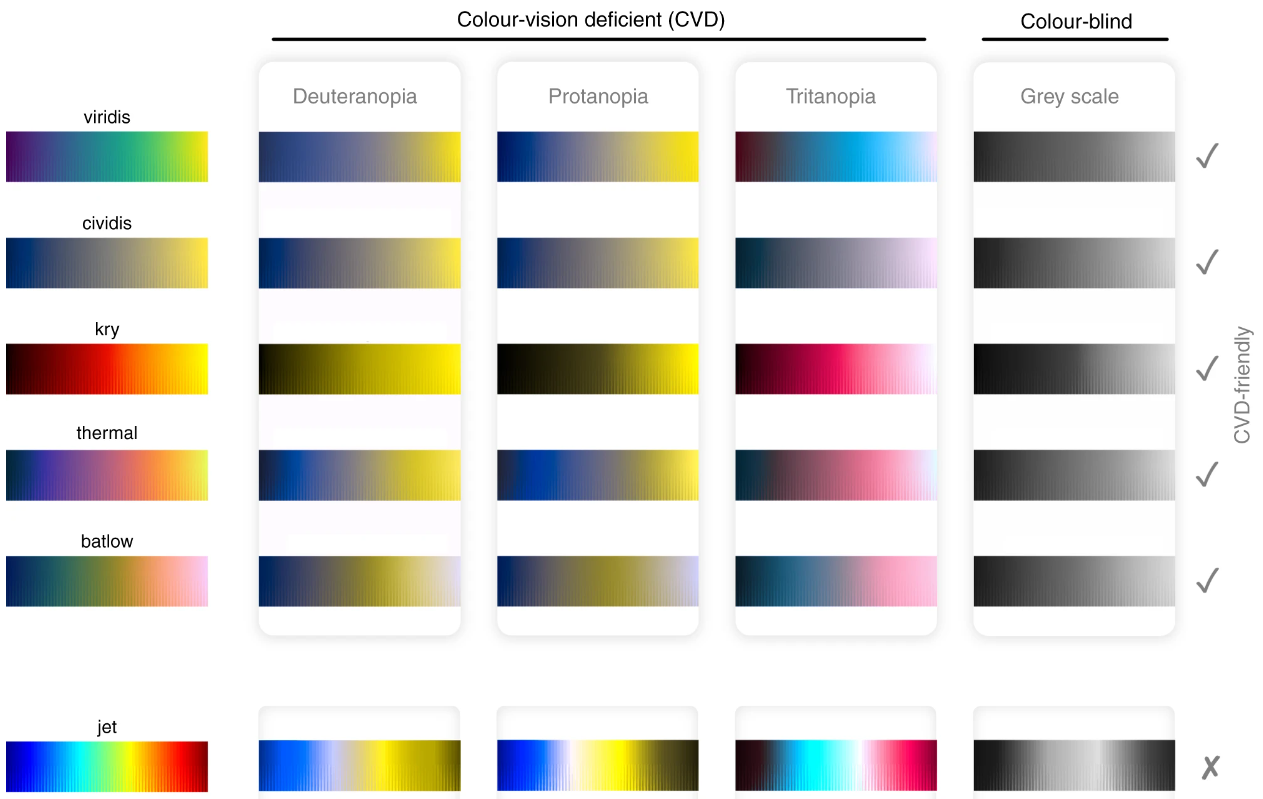
\includegraphics[width=\textwidth]{Photos/Figures/gradients.png}
	\caption{How common gradients appear to various colourblind diagnoses, adapted from \citeauthor{colourScienceMisuse} \cite{colourScienceMisuse}.}
	\label{fig:gradientExample}
	\hfill
\end{figure}



\begin{figure}[hbt!]
	\centering
	\captionsetup{width=0.5\textwidth}
	\def\svgwidth{0.55\textwidth}
	\input{Photos/Figures/MUFASAandGoJettandTranceRelationshipComparison-InverseTimeConstant-MachNumber-2column_Editted.eps_tex}
	\caption{MUFASA B aerodynamic design and coordinate system \cite{BenThesis}. Notice how different symbols and colours are used. Also note how the ends of the x and y axes are denoted by a number and not left ambiguously floating.}
	\label{fig:dataExample}
	\hfill
\end{figure}

\subsubsection{Equations}

Equations are similar to figures and tables in that they are addressed in-text prior to their presentation. 
Unless otherwise stated, the first time a variable is used in an equation it is presented in-text before or just after the equation. 
Exceptions to the rule do exist inline with formatting guidelines specific to the conference/journal/thesis being written. 
An example equation highlighting how aerodynamic forces are added is presented in \cref{eqn:netForce}, 

\begin{equation} \label{eqn:netForce}
	F_{\text{net}} = F_{\text{aero}} + F_{\text{g}} + F_{\text{T}}
\end{equation}

\noindent where $F_{\text{net}}$, $F_{\text{aero}}$, $F_{\text{g}}$, and $F_{\text{T}}$ represent net force, aerodynamic force, gravitational force, and thrust force, respectively. 

\subsection{General Writing}

Common writing mistakes and misconceptions are presented in this section. It is the authors hope this list is useful (and error-free). 
Great writing resources are found online \cite{writingAIAA}, and at the University of Calgary \cite{writingUofC,writingCoursesUofC}. 
The \citeauthor{writingUofC} \cite{writingUofC} in particular is a great resource for 1-on-1 writing help and support, with extremely knowledgeable staff. 
It is strongly recommended to seek assistance \textbf{BEFORE} completing a document. By requesting feedback early, more time can be spent writing properly instead of editing what has already been written. 

\subsubsection{Sentence Structure}
Conciseness is key in academic writing, readers ``want to find the relevant information quickly and efficiently,'' \cite{writingSpringer}. 
Sentences should only contain \textbf{one idea}, and be no longer than 20-25 words in length \cite{writingSpringer}. 


\subsubsection{Language}

A conference/journal/thesis requires exact language be used. 
Using words such as \textit{can}, \textit{could}, and \textit{would} make the document sound uncertain. 
This type of uncertain wording should only be used when discussing future work, which is always inherently uncertain. 
Do not write "\textit{...this can be seen in Fig...,}", instead write "\textit{...this is presented in Fig...}".

A word on the use of the word \textit{this}. 
The word \textit{this} should not start a sentence unless it is followed directly with an indication of what \textit{this} is. 
A sentence should be a standalone idea, thus, without reiterating to the reader what \textit{this} is, it is very easy for the reader to become confused. 
Parallel to this concept of the uncertainty of \textit{this} is how authors sometimes use \textit{it} without explaining what \textit{it} is they are referring to. 

Word choice is paramount and matters. While often used interchangeably in normal language, \textit{compute}, \textit{evaluate}, and \textit{calculate} suggest very different approaches were taken. Consider what verbs are being used throughout the document and what they imply. 


\subsubsection{Commas}

Always use the Oxford comma when making a list. The Oxford comma helps the reader understand if the last two items in a list are together or separate. 

Commas should also be used after transition words, such as ``..., however,...''. 


\subsection{Referencing}

Referencing is a vital part of science, a way to track that all scientific statements are supported by evidence \cite{referncingVirtues}. 
It is imperative that references are used properly and correctly associated to the factual information they are related to. 
As stated by \citeauthor{referncingVirtues} \cite{referncingVirtues}:
\begin{quotation}
	\noindent
	A reference citation is supposed to provide accurate underpinning for a statement and to represent the current state of research, or, in the case of a maverick opinion, to ensure it is recognizable as such. \cite{referncingVirtues}
\end{quotation} 

\noindent
Some good rules of thumb to guide if you need to reference a statement are: 
\begin{itemize}
	\item Did you perform the task/experiment?
	\item If commenting about an industry trend, do you have years of first-hand experience in that industry?
	\item Is the statement common knowledge (ie. it is a first year taught engineering concept/fact)?
	\item Did you develop this equation, figure, diagram? 
	\item Was the idea, method, statement learnt from another source (ie. a textbook or article)?
\end{itemize}
\noindent
If the answer to any of the first four is no, or the last is yes, then you \textbf{NEED} a reference. 
If a reference cannot be found to support a statement, either the statement is incorrect, or it is too broad and should be reworded to be more defensible. 

References are placed at the end of a sentence if describing a single idea, if describing multiple ideas, referencing is placed just behind the idea it is associated with. 
Proper referencing is also a topic formally covered by the \citeauthor{writingUofC} \cite{writingUofC} and \citeauthor{writingCoursesUofC} \cite{writingCoursesUofC}.